% !TeX root = physique.tex
\chapter{Lois de Descartes -- Prisme}
\label{chap:loisdedescartes}
\minitoc
\minilof
\minilot

\section{Nature de la lumière}
\label{chap6-sec:naturedelalumiere}

\subsection{Vitesse de propagation, indices de réfraction}
\label{chap6-subsec:vitessedepropagation}

Une onde progressive électromagnétique monochromatique est constituée d'un champ électrique $\vv{E}$ et d'un champ magnétique $\vv{B}$ vibrant en phase, perpendiculairement entre eux et perpendiculairement à la direction de propagation. 
Si la fréquence de la radiation électromagnétique est $\nu$, alors la période est $\tau = \frac{1}{\nu}$. Si la vitesse de propagation est $v$, la longueur d'onde (période spatiale) est la distance dont l'onde progresse en une période $\lambda = v \tau$. Dans le vide $\lambda_0 = \frac{c}{\nu}$.

Pour un milieu isotrope, homogène, où la vitesse de propagation est $v$, l'indice de réfraction absolu du milieu pour la fréquence $\nu$ est $N = \frac{c}{v}$, $\lambda =  \frac{\lambda_0}{N}$.

Pour deux milieux 1 et 2, homogènes et optiquement isotropes, l'indice de réfraction du milieu 2 par rapport au milieu 1 est le rapport $n_{2/1}= \frac{v_1}{v_2}=\frac{N_2}{N_1}$. Les indices de réfraction dépendent de la fréquence de la radiation considérée.

\subsection{Différents domaines des ondes électromagnétiques}
\label{chap6-subsec:domainesdesondes}

Suivant la longueur d'onde dans le vide, on distingue différents domaines de radiation. La lumière visible correspond à une longueur d'onde dans le vide $\lambda_0$ telle que
\begin{equation}
  \SI{400}{nm} < \lambda_0 < \SI{750}{nm}.
\end{equation}

On distingue différentes couleurs, dans l'ordre des longueurs d'onde croissante~: violet, indigo, bleu, vert, jaune, orangé, rouge. Aux longueurs d'ondes dans le vide inférieure à $\SI{400}{nm}$ jusqu'à environ $\SI{1}{nm}$, on trouve le domaine de l'ultraviolet, puis les rayons $X$, les rayons $\gamma$ et les rayons cosmiques. Aux longueurs d'ondes au-delà de $\SI{750}{nm}$ jusqu'à environ $\SI{1}{mm}$, on trouve le domaine de l'infrarouge, puis celui des ondes radioélectriques.

Dans le domaine de la lumière proprement dite, des ultraviolets et des infrarouges l'indice absolu d'un milieu est toujours supérieur à $1$ et la vitesse de la lumière dans l'air et voisine de $c$. On utilise couramment les indices par rapport à l'air ($n$) au lieu des indices absolus ($N$). 

\section{Propagation rectiligne}
\label{chap6-sec:propagationrectiligne}

\subsection{Hypothèse de propagation rectiligne}
\label{chap6-subsec:hypothesedepropagationrectiligne}

Toute l'optique géométrique repose sur l'hypothèse de la propagation rectiligne de la lumière issue d'une source ponctuelle dans le cas d'une propagation homogène. Cette hypothèse est remise en question par les phénomènes de diffraction qui deviennent appréciable chaque fois que la lumière doit passer dans des fentes dont la largeur est du même ordre (ou inférieure) que la longueur d'onde.

\subsection{Rayons lumineux}
\label{chap6-subsec:rayonslumineux}

\begin{defdef}
 Le trajet rectiligne de la lumière issue d'un point est un rayon lumineux.
\end{defdef}

Un faisceau isogène est formé par des rayons lumineux issu d'un point source. S'il est étroit, on parle de pinceau lumineux. Si la lumière est issue d'une source étendue, on a un faisceau complexe forme une infinité de faisceaux isogènes.

Les phénomènes de réflexion et de réfraction permettant de modifier la direction des rayons lumineux, on peut avoir des faisceaux lumineux divergents, convergents ou cylindriques.

\section{Lois de Descartes}
\label{chap6-sec:LoisdeSnellDescartes}

\subsection{Définitions}
\label{chap6-subsec:définitions}

Elles précisent le comportement d'un rayon lumineux arrivant sur une surface réfléchissante et réfringente $\Sigma$ séparant deux milieux de propagation homogènes et isotropes.

On appelle point d'incidence le point d'intersection du rayon incident avec la surface $\Sigma$. La normale à $\Sigma$ en ce point et le rayon d'incidence déterminent le plan d'incidence. L'angle entre la normale au point d'incidence et le rayon incident est l'angle d'incidence. Il y a deux rayons émergents. Le rayon émergent dans le même mileu que le rayon incident est le rayon réfléchi, et l'angle qu'il forme avec la normale au point d'incidence est l'angle de réflexion. Le rayon émergent dans le second milieu de propagation est le rayon réfracté, l'angle qu'il forme avec la normale au point d'incidence s'appelle l'angle de réfraction.

\begin{theo}[Lois de Descartes pour la réflexion]
  Le rayon réfléchi appartient au plan d'incidence. L'angle de réflexion est égal à l'angle d'incidence : $i'=i$.
\end{theo}
\begin{theo}[Lois de Descartes pour la réfraction]
  Le rayon réfracté appartient au plan d'incidence. L'angle de réfraction $i_2$ est tel que $n_1 \sin i_1 = n_2 \sin i_2$, en notant $i_1$ l'angle d'incidence et $n$ l'indice des milieux.
\end{theo}

On remarquera que si une lumière monochromatique donnée est plus freinée par le milieu 2 que par le milieu 1, on dit que le milieu 2 est plus réfringent que le milieu 1. Dans ce cas, $v_2 < v_1$ (ou $n_2 > n_1$), et il en résulte que $i_2 > i_1$.

Si le milieu 2 est plus réfringent que le milieu 1, le rayon lumineux se rapproche de la normale lors du passage de la lumière.

\begin{theo}[Loi du retour inverse]
  Le trajet suivi par la lumière n'est pas modifié si le sens de propagation est inversé.
\end{theo}

\subsection{Réflexion totale et réfraction limite}
\label{chap6-subsec:reftotale}
Soit un rayon lumineux passant du milieu 1 au milieu 2 plus réfringent ($n_{2/1}>1$). L'angle de réfraction est tel que $n_{2/1} \sin i_2 = \sin i_1$, donc
\begin{equation}
  i_2 < \arcsin \left(\frac{1}{n_{2/1}} \right) = i_m.
\end{equation}
L'angle limite de réfraction $i_m$ correspond à un rayon incident longeant la surface réfringente ($i_1 = \frac{\pi}{2}$).

Inversement, si la lumière passe du milieu 2 (plus réfringent) au milieu 1 (moins réfringent), l'angle d'incidence $i_2$ ne dépassera pas la valeur $i_m$ obtenue pour un angle de réfraction $i_1 = \frac{\pi}{2}$. Si l'angle d'incidence est supérieur à $i_m$, il y a réflexion totale.

Par exemple, si un verre a l'indice $n=\frac{3}{2}$ par rapport à l'air, pour une lumière monochromatique donnée, l'angle limite de réfraction pour le passage de la lumière de l'air au verre (ou l'angle d'incidence à partir duquel il y a réflexion totale pour le passage du verre à l'air) est $i_m = \arcsin\left(\frac{2}{3}\right) = 41,8$
 degrés.
\section{Prisme}
\label{chap6-sec:prisme}

Un prisme est un mileu transparent, homogène et optiquement isotrope, limité par deux faces planes et une base. On s'intéressera uniquement ici à un prisme placé dans l'air et éclairé en lumière monochromatique.

Le rectiligne du dière formé par les deux faces planes est nommé angle du prisme, noté souvent $A$. L'indice du mileu transparent par rapport à l'air est l'indice du prisme, noté $n$. Il dépend de la longueur d'onde dans le vide de la lumière. On s'intéresse uniquement ici au cas d'un rayon incident contenu dans un plan de section droite du prisme, c'est-à-dire dans un plan perpendiculaire à l'arête du dièdre.

La première loi de Descartes pour la réfraction implique que le trajet d'un tel rayon lumineux se fera entièrement dans un plan de section principale constitué par le plan d'incidence sur la face d'entrée.

L'angle d'incidence sur la face d'entrée sera noté $i$ et l'angle de réfraction sur la face de sortie $i'$. L'angle $i$ est compté positivement lorsque le rayon incident est du même coté de la normale à la face d'entrée que la base du prisme et négativement s'il est du même côté que l'arête. De même pour l'angle $i'$, il est positif si le rayon émergeant est du même côté de la normale à la face de sortie que la base du prisme et négativement dans l'autre cas.

L'angle de réfraction sur la face d''entrée sera noté $r$ et l'angle d'incidence sur la face de sortie sera noté $r'$. Les angles $r$ et $r'$ sont comptés positivement pour des rayons correspondants situés du même côté de la normale correspondante que l'arête du prisme.

\subsection{Les formules du prisme}
\label{chap6-subsec:formulesprisme}

Les deux premières formules traduisent la deuxième loi de Descartes pour la réfraction : $\sin(i) = n\sin(r)$ et $\sin(i') = n\sin(r')$. Les deux autres sont géométriques : $r+r'=A$ et $D=i+i'-A$. $D$ est la déviation, c'est l'angle entre le rayon incident et le rayon émergeant. \emph{Un rayon lumineux est toujours dévié vers la base du prisme, $D \geq 0$}.

\subsection{Étude de la déviation en fonction de l'angle d'incidence}
\label{chap6-subsec:etudedeviation}
\paragraph{Existence d'un minimum de déviation}

Pour une lumière monochromatique donnée et un prisme donnée, $n$ et $A$ sont constants. Les formules du prisme donnent alors:
$r = \arcsin{\frac{\sin(i)}{n}}$ et donc $r'=A - \arcsin{\frac{\sin(i)}{n}}$ et donc aussi $i' = \arcsin n\sin (A-\arcsin(\sin(i)/n))$, donc finalement~:
\begin{equation}
  D = i + \arcsin{n\sin\left(A-\arcsin{\frac{\sin(i)}{n}}\right)} -A.
\end{equation}
Cette fonction, $D=f(i)$ est assez compliquée à étudier, mais on peut montrer qu'elle admet un seul extremum, qui est d'ailleurs un minimum. On peut le confirmer par expérience.

\paragraph{Symétrie au minimum de déviation}

La loi du retour inverse de la lumière implique que si $i$ prend la valeur $i_1$ et $i'$ la valeur $i_2$ pour un sens donné de la lumière, alors, pour le sens inverse, $i=i_2$ et $i'=i_1$. La déviation est la même pour les deux sens de la lumière. Donc, à chaque valeur de $D$, il correspond deux angles d'incidence possibles. Mais au minimum de déviation $D_m$ il n'en correspond qu'un seul.

Pour $D=D_m$, on a $i=i'$ et par conséquent $r=r'$, \emph{la figure est alors symétrique par rapport au plan bisecteur du dièdre formé par le prisme.} En indiçant par $m$ les valeurs correspondantes au minimum de déviation, on a~: $r_m = r'_m = \frac{A}{2}$, $D_m = 2i_m-A$, d'où $i_m = \frac{D_m+A}{2}$ ; avec $\sin(i_m) = n\sin(r_m)$, on obtient~:
\begin{equation}
	n = \frac{\sin\left(\frac{D_m+A}{2}\right)}{\sin\left(\frac{A}{2}\right)}
\end{equation}

\paragraph{Déviation maximale, condition d'émergence}

Un rayon lumineux pou\-rra de toute façon traverser la face d'entrée du prisme quel que soit son angle d'incidence, mais il ne traversera la face de sortie que si son angle d'incidence $r'$ sur celle-ci est inférieur à $i_m = \arcsin 1/n$ ce qui correspond à $i'_0 = \frac{\pi}{2}$ et à $r_0 = A - \arcsin 1/n$ donc à l'angle d'incidence minimal $i_0 = \arcsin(n\sin(A-\arcsin 1/n))$. On remarquera que cet angle peut être positif ou négatif suivant la valeur du prisme $A$. La déviation prendra alors sa valeur maximale, la même que pour $i=\frac{\pi}{2}$, d'après la loi du retour inverse de la lumière~:\begin{equation}
	D_m = i_0 +\frac{\pi}{2} - A
\end{equation}

\subsection{Exemple}
\label{chap6-subsec:exemple}
Soit un prisme d'angle au sommet $A = \frac{\pi}{6}$, d'indice $n=\frac{3}{2}$ pour une lumière monochromatique considérée.

Au minimum de déviation, $r=r'=r_m=\frac{A}{2}=\frac{\pi}{12}$, et $i=i'=i_m=\arcsin\left(\frac{3}{2}\sin(\pi/12)\right) = \arcsin\left(\frac{3}{2} \frac{\sqrt{2-\sqrt{3}}}{2}\right)$ soit 22.8 degrés, et $D_m=2i_m-A$ vaut approximativement 15.7 degrés.
L'angle d'incidence minimal permettant la traversée de la deuxième face du prisme est $i_0$ tel que $i'_0=\frac{\pi}{2}$, d'où $r'_0 = \arcsin(1/n)$ soit approximativement 41.8 degrés et $r_0=A-r'_0$ soit -11.8 degrés d'où $i_0=\arcsin(1.5 \sin(r_0))$ soit approximativement -17.9 degrés. La déviation maximale est donc de $D_0 = i_0 + \frac{\pi}{2}-A$ approximativement 42.1 degrés. Elle est obtenue pour $i=i_0$ et $i'=\frac{\pi}{2}$ comme pour $i=\frac{\pi}{2}$ et $i'=i_0$.

Pour $i=0$ on a $r=0$, $r'=A=\frac{\pi}{6}$. On a alors $i'=\arcsin(\frac{3}{2}\sin(\pi/6))$ soit approximativement 48.6 degrés et une déviation $D=i'-A$ soit approximativement 18.6 degrés. La même déviation est obtenue pour $i$ valant 48.6 degrés et $i'=0$.
Le tracé complet de $D=f(i)$ est réalisé ci-dessous sur la figure \ref{fig:chap6-deviation}, directement avec l'expression de cette fonction.
\begin{figure}
	\centering
	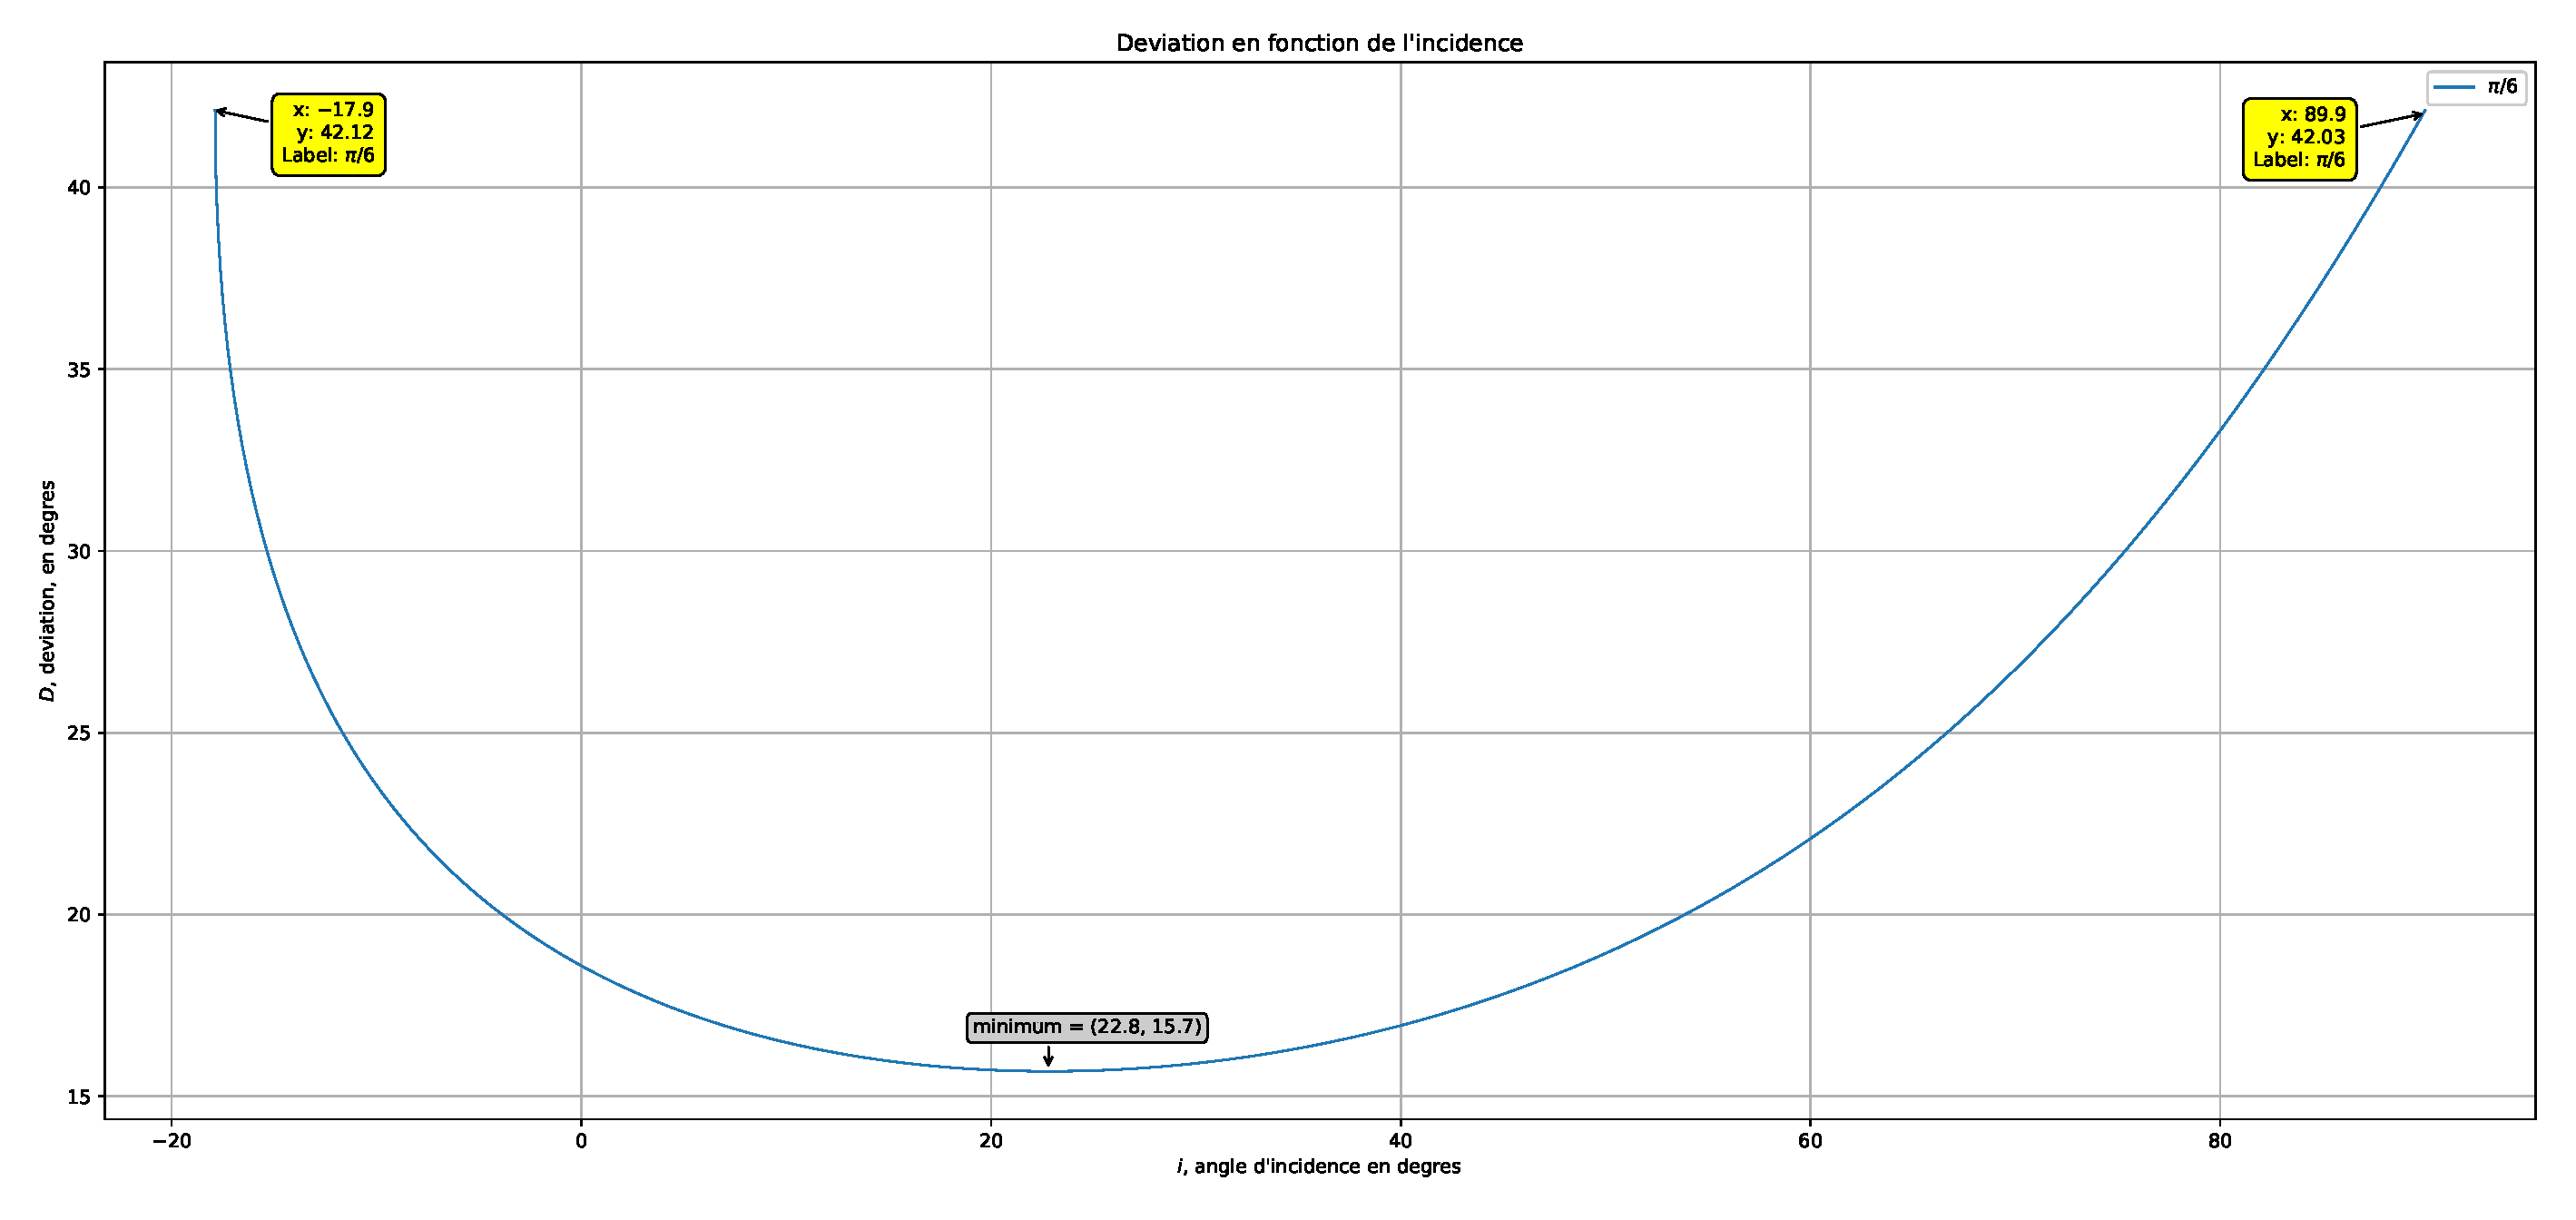
\includegraphics[width=\textwidth]{Deviation_optique.eps}
	\caption{Deviation en fonction de l'incidence}
	\label{fig:chap6-deviation}
\end{figure}
\subsection{Étude de la déviation, dispersion polychromatique}

On retiendra d'abord que \emph{l'indice d'un milieu transparent estune fonction croissante de la fréquence de la lumière, donc décroissante en fonction de la longueur d'onde dans le vide}.

En effet, pour les radiations lumineuse (aussi dans l'infrarouge et l'ultraviolet), mais pas au delà,\emph{la lumière est d'autant plus freinée que ses photons ont plus d'énergie}, donc si $E=h \nu$ croît, alors la longueur d'onde dans le vide $\lambda_0 = h/\nu$ décroît, la vitesse $v$ décroît et donc l'indice de réfraction par rapport à l'aire $n=c/v$ croît. À la lumière violette correspond un indice plus élevé que pour la lumière rouge.

Il en réslte qu'un rayon entrant dans un milie moins réfringent est d'autant plus dévié (rapproché de la normale) que sa longueur d'onde dans le vide est basse. De même, un rayon entrant dans u milieu moins réfringent est d'autant plus dévié (écarté de la normale) que lorsque sa longueur d'onde dans le vide est plus basse.

Pour un rayon lumineux traversant le prisme, les deux déviations $i-r$ et $i'-r'$ (dont la somme est $D$) se font dans le même sens, vers la base du prisme ; donc, pour un angle d'incidence fixé, \emph{un rayon lumineu est d'autant plus dévié par un prisme que sa longueur d'onde dans le vide est plus basse.}
\emph{Un prisme permet donc de disperser une lumière polychromatique plus efficacement, grâce aux deux réfractions, qu'un réfraction unique}.

\section{Exercices}

\begin{exercice}[Conditions d'émergences pour le prisme]
	Soit un prisme d'indice $n$, plongé dans l'air d'indice 1, d'angle $A$.
	Soit $S$ la source lumineuse ponctuelle et $SI$ un rayon incident contenu dans un plan de section principale, $I$ étant le point d'incidence. Le rayon réfracté par la première face frappe la seconde face du prisme en $I'$. Le rayon réfracté par la seconde face est $I'R$, lorsqu'il existe.

	On utilisera les notations et les conventions de signes habituelles pour les angles $i$, $i'$, $r$ et $r'$ et $D$.
	\begin{enumerate}
\item Montrer que, lorsqu'il existe, le rayon $I'R$ est dans le plan de section principale de $SI$.
\item Établir les quatre formules du prisme.
\item Montrer que pour que le rayon $I'R$ existe, il est nécessaire que les deux conditions suivantes soient satisfaites : $A \leq 2 \arctan(1/n)$ et $i_0 \leq i \leq \pi/2$ avec $\sin i_0 = n \sin\left(A-\arcsin(1/n)\right)$.
	\end{enumerate}
\end{exercice}

\begin{exercice}[Étude du minimum de déviation]
	Les notations sont celles de l'exercice précédent.
	\begin{enumerate}
		\item
		\begin{enumerate}
			\item Montrer que la déviation $D$ passe par un minimum $D_m$ lorsque $ii=i'=i_m$.
			\item Exprimer l'indice $n$ du prisme en fonction de $A$ et $D_m$.
			\item Tracer l'allure de la courbe de $D=f(i)$. On précisera les tangentes aux deux extrémités $i=i_0$ et $i=\pi/2$, ainsi que la valeur de la déviation $D_0$ correspondante.
			\item Quel est d'après vous l'intérêt d'utiliser le prisme au minimum de déviation ?
		\end{enumerate}
		\item Dans un spectroscope à prisme, le prisme est éclairé en lumière parallèle (donc sous une incidence $i$ fixée), est monochromatique, de longueur d'onde dans le vide $\lambda$, variable. Exprimer $\derived{D}{\lambda}$, en fonction de $\derived{n}{\lambda}$ (dispersion du verre du prisme), $A$, $r$ et $i'$.
		\item On se place au minimum de déviation pour une longueur d'onde $\lambda$ donnée. Le faisceau incident est obtenu grâce à une fente éclairée par la source, parallèle à l'arête du prisme et une lentille convergente $L_1$, de distance focale $f'$, placée entre la fente et le prisme. Le spectre obtenu est recueilli sur une plaque photographique dans le plan focal d'une lentille convergente $L_2$ de même distance focale $f'$ que $L_1$. La base de la partie éclairée du prisme a une largeur $b$, celui-ci est éclairé jusqu'à son arête. Le faisceau émergent a une largeur égale à $a$ dans les plans de section principale du prisme. Exprimer $\derived{D}{\lambda}$ en fonction de $a$, $b$ et $\derived{n}{\lambda}$. 
	\end{enumerate}
\end{exercice}

\begin{exercice}[Fibre optique à saut d'indice]
	Soit une fibre optique $F$ constituée d'un cœur cylindrique de rayon $a$ et d'indice $n_1$, entouré d'une gaine d'indice $n_2 \leq n_1$ et de rayon extérieur $b$. Les faces d'entrées et de sortie sont perpendiculaires au cylindre d'axe $(Oz)$ formé par la fibre. L'ensemble, en particulier la face d'entrée, est en contact avec un milieu d'indice $n_0$ et pour les applications numériques, on considérera que ce milieu est de l'air $n_0=1$.
	\begin{enumerate}
		\item "Zigzag plan". Un rayon lumineux $SI$ arrive en un point $I$ sur la face d'entrée de la fibre. À quelles conditions d'incidence ce rayon a-t-il, dans la fibre, un trajet plan ? 
		
		On considère un rayon $(SI)$ incident sur le cœur et contenu dans le plan $Oxz$. On appelle $i$ l'angle d'incidence et $\theta$ l'angle de la réfraction sur la face d'entrée de la fibre.
		\item Déterminer en fonction de $n_0$, $n_1$ et $n_2$ la condition que doit satisfaire $i$ pour que le rayon réfracté ait une propagation guidée dans le cœur. la valeur maximale de $i$ est alors désignée par $i_a$, l'angle d'acceptance de la fibre.
		\item On appelle ouverture numérique $ON$ du guide la quantité $ON=n_0 \sin i_a$. Exprimer l'ouverture numérique en fonction de $n_1$ et $n_2$.
		\item Calculer $i_a$ et $ON$ pour une fibre d'indice $n_1=1.456$ (silice) et $n_2=1.410$ (silicone). Quelles seraient les valeurs de ces grandeurs pour un guide à base d'arséniure de gallium pour lequel $n_1=3.9$ et $n_2=3$ ? Commenter
		
		L'atténuation de la lumière dans les fibres optiques est due à l'absorption et à la diffusion par le matériau constitutif du cœur et par ses impuretés (les ions fers 2, les ions cuivres 2, les ions hydroxyde, \ldots). Elle se mesure en décibels par kilomètre : $A=\frac{\SI{10}{km}}{l} \log(\Phi_1/\Phi_2)$, où $\Phi_1$ et $\Phi_2$ désignent les flux lumineux (puissance lumineuse) dans les plans de front successifs 1 et 2 distants de $l$.
		
		\item On parvient couramment à réaliser des fibres dans lesquelles le flux, après un parcours de 50 kilomètres, représente 10 pourcents du flux incident. Calculer l'atténuation de telles fibres. Applications : Endoscope à fibres, fibroscope. Le but d'un endoscope est de permettre à un observateur de "voir" dans des endroits inaccessibles, d'intérêts divers (médical, militaire, industriel, \ldots). L'endoscope à fibres est constitué de deux faisceaux de fibres : l'un éclaire le site, l'autre assure le retour vers l'extérieur de la lumière émise par la cible éclairée. Le nombre de fibres constituant chaque faisceau est de l'ordre de 10 mille à 1 million.
		
		\item Si l'on imagine la cible divisée en 100 mille petits carrés à peu près, chaque fibre au voisinage de la cible recueillant la lumière de l'un d'eux, quel est le problème posé à l'autre extrémité par la reconstitution de l'image ? Quel est le problème technologique majeur posé alors par la fabrication d'un faisceau de fibres ?
	\end{enumerate}
	
 
\end{exercice}
